% ============================================================================
%  RODENTNET: MASTER PRESENTATION DECK (LATEX BEAMER - DE-DENSIFIED EDITION)
%  Quantum-Resilient Federated Learning for Private Immunological Sequences
%  Widescreen 16:9 Format | 22 Spacious, Comprehensive Defense Slides
%  Tag: v1.3-audit-final | Commit: 7d9d12e | Deterministic Reproduction
% ============================================================================
\documentclass[aspectratio=169,10pt]{beamer}

% Theme configuration
\usetheme{Madrid}
\usecolortheme{whale}

% Typography & layout
\usepackage{booktabs}
\usepackage{tabularx}
\usepackage{array}
\usepackage{amsmath}
\usepackage{amssymb}
\usepackage{pifont}
\usepackage{listings}
\usepackage{graphicx}
\usepackage{tikz}
\usetikzlibrary{arrows.meta,positioning,shapes.geometric,shadows,calc}

% Color definitions
\definecolor{primaryblue}{RGB}{15, 43, 72}
\definecolor{accentblue}{RGB}{37, 99, 235}
\definecolor{darkteal}{RGB}{6, 95, 70}
\definecolor{crimson}{RGB}{153, 27, 27}
\definecolor{slate}{RGB}{71, 85, 105}
\definecolor{lightbg}{RGB}{248, 250, 252}

\setbeamercolor{palette primary}{bg=primaryblue,fg=white}
\setbeamercolor{palette secondary}{bg=accentblue,fg=white}
\setbeamercolor{palette tertiary}{bg=slate,fg=white}
\setbeamercolor{structure}{fg=accentblue}
\setbeamercolor{frametitle}{bg=primaryblue,fg=white}
\setbeamercolor{block title}{bg=primaryblue,fg=white}
\setbeamercolor{block body}{bg=lightbg,fg=black}
\setbeamercolor{block title example}{bg=darkteal,fg=white}
\setbeamercolor{block body example}{bg=lightbg,fg=black}
\setbeamercolor{block title alerted}{bg=crimson,fg=white}
\setbeamercolor{block body alerted}{bg=lightbg,fg=black}

% Remove navigation symbols
\setbeamertemplate{navigation symbols}{}

% Custom footer
\setbeamertemplate{footline}{
  \leavevmode%
  \hbox{%
  \begin{beamercolorbox}[wd=.333333\paperwidth,ht=2.25ex,dp=1ex,center]{author in head/foot}%
    \usebeamerfont{author in head/foot}Harishankar S \& Team (Group 8)
  \end{beamercolorbox}%
  \begin{beamercolorbox}[wd=.333333\paperwidth,ht=2.25ex,dp=1ex,center]{title in head/foot}%
    \usebeamerfont{title in head/foot}RodentNet: Post-Quantum SecAgg
  \end{beamercolorbox}%
  \begin{beamercolorbox}[wd=.333333\paperwidth,ht=2.25ex,dp=1ex,right]{date in head/foot}%
    \usebeamerfont{date in head/foot}\insertframenumber{} / \inserttotalframenumber\hspace*{2ex}
  \end{beamercolorbox}}%
  \vskip0pt%
}

% Code style
\lstdefinestyle{code}{
  basicstyle=\ttfamily\scriptsize,
  breaklines=true,
  frame=single,
  backgroundcolor=\color{black!3}
}

% Metadata
\title[RodentNet: Quantum-Resilient SecAgg]{RODENTNET: QUANTUM-RESILIENT SECURE FEDERATED LEARNING}
\subtitle{Authenticated Post-Quantum Signatures, Finite-Field MPC, and Neural Sequence Modeling on Private TCR Repertoires}
\author[Harishankar S et al.]{Harishankar S \& Team (Group 8)\\[0.1cm]{\small Technical Advisory: Dr. Thushara A \& Mr. Gokul Alex}}
\institute[Dept. of CSE]{Department of Computer Science and Engineering\\[0.1cm]{\footnotesize Repository State: Commit \texttt{7d9d12e} (\texttt{v1.3-audit-final})}}
\date{Final Project Defense \& Review}

% ============================================================================
\begin{document}

% ----------------------------------------------------------------------------
% SLIDE 1: Title Slide
% ----------------------------------------------------------------------------
\begin{frame}[plain]
  \titlepage
\end{frame}

% ----------------------------------------------------------------------------
% SLIDE 2: Executive Summary & Empirical Highlights
% ----------------------------------------------------------------------------
\begin{frame}{Executive Summary: Audited Empirical Highlights}
  \begin{columns}[T]
    \begin{column}{0.48\textwidth}
      \begin{block}{Statistically Verified Utility Gain}
        \textbf{+6.21 $\pm$ 5.11 pp} paired gain over isolated hospital training ($p = 0.00397$, 10 random seeds). Positive gain in 9 of 10 seeds.
      \end{block}
      \begin{block}{Exact Mathematical Parity}
        \textbf{0.00\%} empirical utility degradation ($\max|\Delta\theta| \le 2.4 \times 10^{-7}$). Float precision preserved via 40-bit prime $\mathbb{Z}_p$.
      \end{block}
    \end{column}
    \begin{column}{0.48\textwidth}
      \begin{block}{Bounded Bandwidth Overhead}
        Steady-state uplink coordination adds strictly \textbf{$<3.86\%$} ($47.48$\,KiB at $N=50$). Post-quantum increment is $+3.15$\,KiB ($<0.26\%$).
      \end{block}
      \begin{block}{Demonstrated Privacy Shield}
        Shadow-dataset MIA AUROC collapses from \textbf{$0.578 \to 0.515$} ($p = 0.0012$, 20 seeds), indistinguishable from pure noise ($0.486$).
      \end{block}
    \end{column}
  \end{columns}
\end{frame}

% ----------------------------------------------------------------------------
% SLIDE 3: Clinical Motivation & Genomic Privacy Challenge
% ----------------------------------------------------------------------------
\begin{frame}{Clinical Motivation: Private Immunological Sequences}
  \begin{columns}[T]
    \begin{column}{0.5\textwidth}
      \begin{block}{TCR Biological Fingerprints}
        \begin{itemize}[itemsep=4pt]
          \item T-cell receptor (TCR) CDR3 loops are hypervariable sequences formed by somatic V(D)J recombination.
          \item Function as \textbf{individual genetic barcodes} revealing infection history, cancer status, and autoimmune profiles.
          \item Cannot be anonymized without destroying immunological predictive structure.
        \end{itemize}
      \end{block}
    \end{column}
    \begin{column}{0.5\textwidth}
      \begin{block}{Decentralized Clinical Dilemma}
        \begin{itemize}[itemsep=4pt]
          \item Clinical centers hold isolated, sample-sparse cohorts of antigen-specific clonotypes.
          \item Data pooling prohibited under \textbf{HIPAA, GDPR}, and biomedical privacy regulations.
          \item Local training fails due to severe non-IID label skew (modeled via Dirichlet $\alpha = 0.5$).
        \end{itemize}
      \end{block}
    \end{column}
  \end{columns}
\end{frame}

% ----------------------------------------------------------------------------
% SLIDE 4: The Three Compounding Threat Vectors
% ----------------------------------------------------------------------------
\begin{frame}{Problem Formulation: The Three Compounding Threats}
  \begin{columns}[T]
    \begin{column}{0.33\textwidth}
      \begin{alertblock}{1. Genomic Privacy Breach}
        \footnotesize
        \textbf{Gradient Inversion:}\\
        Uploading plaintext model weights allows semi-honest servers to invert parameter gradients and recover private CDR3 sequences.\\
        \vspace{0.1cm}
        \textbf{Empirical Leakage:}\\
        Plain FL leaks membership with AUROC $0.578$ and positive cosine correlation ($+0.259$).
      \end{alertblock}
    \end{column}
    \begin{column}{0.33\textwidth}
      \begin{alertblock}{2. The Quantum Threat}
        \footnotesize
        \textbf{Shor's Algorithm:}\\
        Classical cryptosystems (ECDH, RSA, Ed25519) will be cracked in polynomial quantum time.\\
        \vspace{0.1cm}
        \textbf{Harvest Now, Decrypt Later:}\\
        Adversaries record encrypted clinical communications today to expose patient genomes when CRQCs arrive in 10--15 years.
      \end{alertblock}
    \end{column}
    \begin{column}{0.33\textwidth}
      \begin{alertblock}{3. Edge Network Dropouts}
        \footnotesize
        \textbf{Stranded Noise Masks:}\\
        In pairwise masking, Client A adds $+s$ and Client B subtracts $-s$. If Client B disconnects, $+s$ is permanently stranded.\\
        \vspace{0.1cm}
        \textbf{Convergence Failure:}\\
        Without dynamic unmasking, stranded noise ruins aggregation, corrupting global training.
      \end{alertblock}
    \end{column}
  \end{columns}
\end{frame}

% ----------------------------------------------------------------------------
% SLIDE 5: Literature Review & Taxonomy Matrix
% ----------------------------------------------------------------------------
\begin{frame}{Literature Review: Where Does RodentNet Stand?}
  \small
  \begin{table}[h]
    \centering
    \scriptsize
    \begin{tabular}{@{}p{2.8cm}ccccc@{}}
      \toprule
      \textbf{Framework} & \textbf{PQC Secure?} & \textbf{Asym KEM?} & \textbf{Dropout Tolerant?} & \textbf{Uplink Overhead} & \textbf{Bio Validated?} \\
      \midrule
      \textbf{Plain FedAvg} (2017)      & \ding{55} None & N/A & \ding{51} Yes & 0.0\% (1.0$\times$) & Synthetic / Text \\
      \textbf{SecAgg} (Bonawitz 2017)   & \ding{55} Diffie-Hellman & \ding{55} DH only & \ding{51} Shamir on sk & $O(N)$ Shares & Synthetic Data \\
      \textbf{SecAgg+} (Choi 2020)      & \ding{55} Classical & \ding{55} Symmetric & \ding{51} Graph Shamir & $O(\log N)$ & Synthetic Data \\
      \textbf{Cheetah} (Huang 2021)     & \ding{51} LHE / Ring & \ding{55} LHE only & \ding{55} Complex HE & $20\times\text{--}100\times$ & Vision Datasets \\
      \textbf{Assisting-Node PQC} (2025) & \ding{51} Kyber/Dilithium & \ding{51} Kyber768 & \ding{51} Assisting Node & Third-Party Node & MNIST / Toy \\
      \midrule
      \textbf{RODENTNET (This Work)}     & \textbf{\ding{51} FIPS 203/204} & \textbf{\ding{51} ML-KEM-768} & \textbf{\ding{51} Model B Shamir} & \textbf{$< \mathbf{3.86\%}$} & \textbf{\ding{51} Human TCR (VDJdb)} \\
      \bottomrule
    \end{tabular}
  \end{table}
  \begin{block}{Key Distinction}
    \footnotesize
    RodentNet is the first framework combining NIST post-quantum standards with finite-field zero-sum masking and Model B Shamir sharing, eliminating $100\times$ homomorphic expansion and third-party assisting nodes while proving zero utility loss on real clinical TCR sequences.
  \end{block}
\end{frame}

% ----------------------------------------------------------------------------
% SLIDE 6: End-to-End System Topology (Embedded Graphic)
% ----------------------------------------------------------------------------
\begin{frame}{System Architecture: End-to-End Network Topology}
  \begin{columns}[c]
    \begin{column}{0.58\textwidth}
      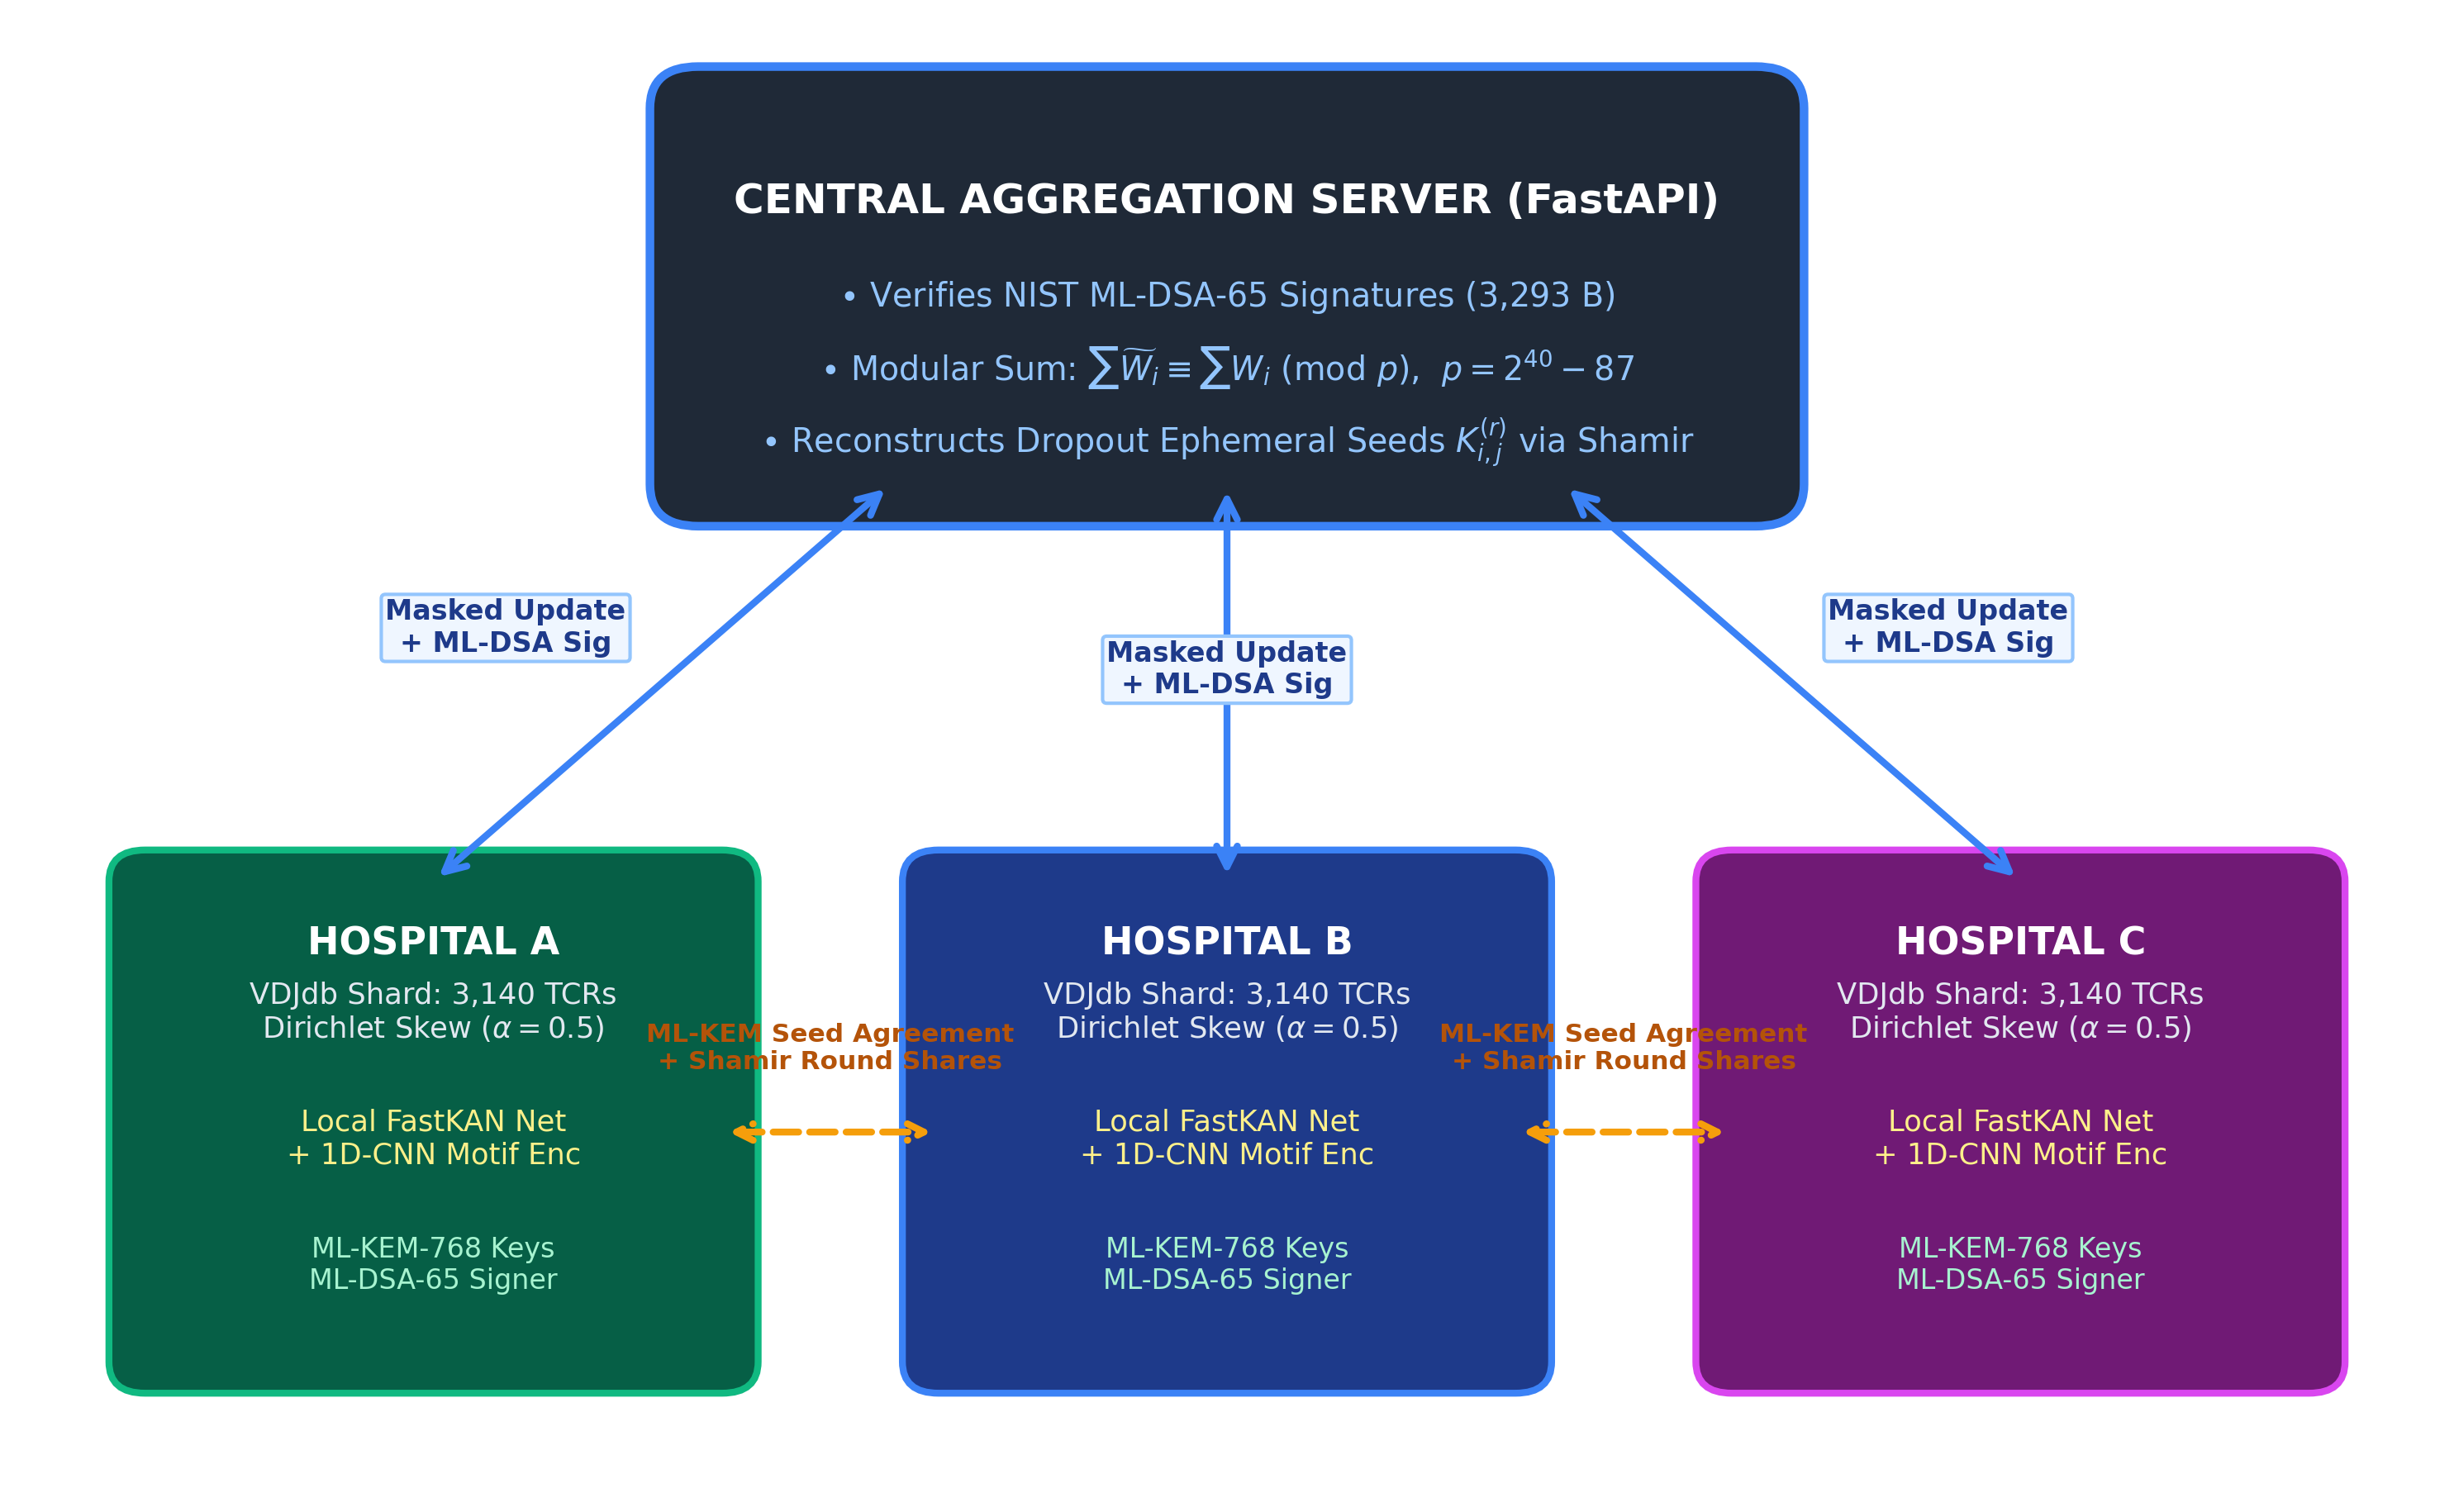
\includegraphics[width=\textwidth]{figures/system_topology_architecture.png}
    \end{column}
    \begin{column}{0.42\textwidth}
      \begin{block}{Central Orchestrator (FastAPI)}
        \scriptsize
        \begin{itemize}[itemsep=2pt]
          \item Verifies 3,293-byte NIST ML-DSA-65 client signatures.
          \item Executes modular zero-sum accumulation in $\mathbb{Z}_p$.
          \item Coordinates dynamic dropout unmasking via Lagrange interpolation.
        \end{itemize}
      \end{block}
      \begin{block}{Hospital Edge Nodes (A, B, C)}
        \scriptsize
        \begin{itemize}[itemsep=2pt]
          \item Private non-overlapping TCR shards (Dirichlet $\alpha=0.5$).
          \item Trains local FastKAN sequence model.
          \item Applies anti-symmetric Galois field blinding before uplink.
        \end{itemize}
      \end{block}
    \end{column}
  \end{columns}
\end{frame}

% ----------------------------------------------------------------------------
% SLIDE 7: Methodology Pipeline Flow (Embedded Graphic)
% ----------------------------------------------------------------------------
\begin{frame}{Methodology Pipeline: Full-Stack Execution Workflow}
  \centering
  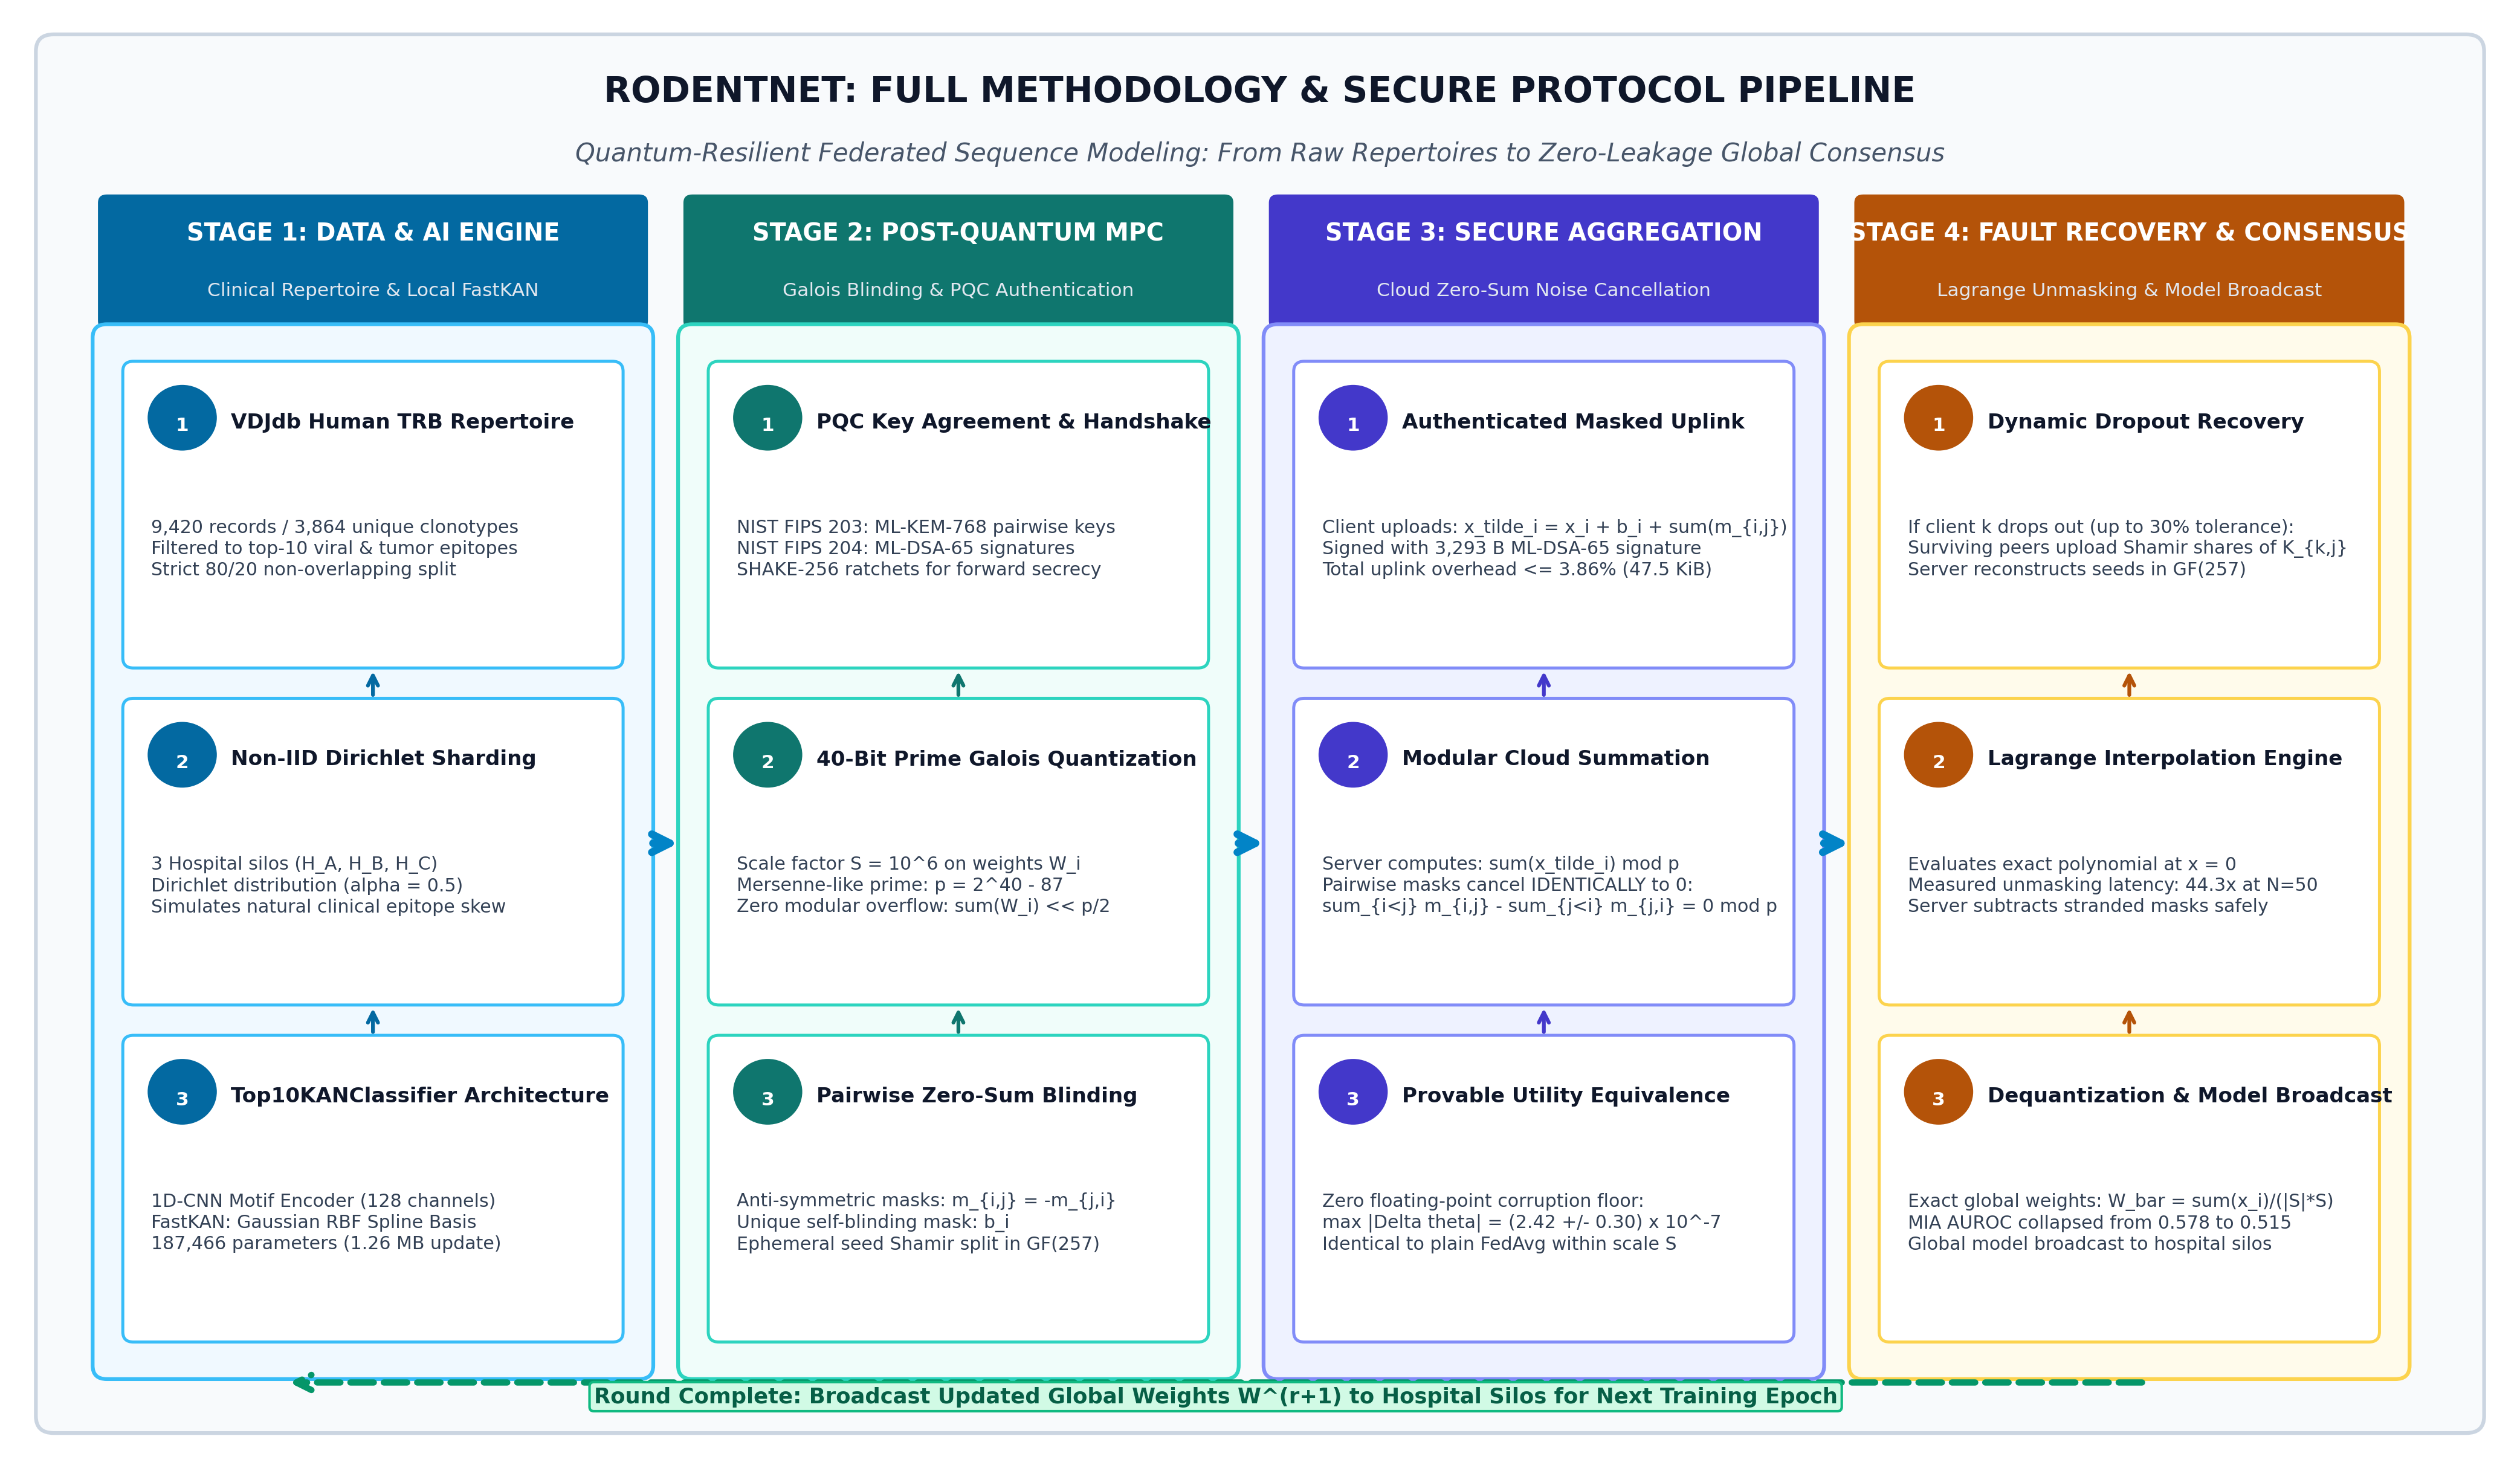
\includegraphics[width=0.95\textwidth]{figures/methodology_pipeline_flow.png}
\end{frame}

% ----------------------------------------------------------------------------
% SLIDE 8: Local AI Model: Top10KANClassifier
% ----------------------------------------------------------------------------
\begin{frame}{Local AI Sequence Engine: Top10KANClassifier Architecture}
  \begin{columns}[T]
    \begin{column}{0.52\textwidth}
      \begin{block}{Neural Processing Pipeline}
        \small
        \begin{itemize}[itemsep=3pt]
          \item \textbf{Input:} CDR3$\beta$ sequences padded to $L=30$, one-hot encoded into $30 \times 20$ amino acid representation.
          \item \textbf{Motif Detection:} Two sequential 1D-CNN layers (128 channels, $k=3$) extracting local tripeptide patterns and structural anchors.
          \item \textbf{FastKAN Spline Head:} Kolmogorov-Arnold Network with learnable Gaussian RBF basis functions capturing localized biochemical interactions.
          \item \textbf{Linear Logits:} Projection to 10 viral/tumor epitope classes.
        \end{itemize}
      \end{block}
    \end{column}
    \begin{column}{0.48\textwidth}
      \begin{table}[h]
        \centering
        \scriptsize
        \begin{tabular}{@{}lcc@{}}
          \toprule
          \textbf{Layer / Component} & \textbf{Output Shape} & \textbf{Parameters} \\
          \midrule
          Input Embedding    & $(B, 20, 30)$   & 0 \\
          Conv1D Layer 1     & $(B, 128, 28)$  & 7,808 \\
          Conv1D Layer 2     & $(B, 128, 26)$  & 49,280 \\
          FastKAN Spline     & $(B, 64)$       & 130,048 \\
          Linear Classifier  & $(B, 10)$       & 330 \\
          \midrule
          \textbf{Total Model} & \textbf{187,466} & \textbf{1.26 MB Update} \\
          \bottomrule
        \end{tabular}
      \end{table}
      \begin{exampleblock}{FastKAN Spline Advantage}
        \scriptsize
        Gaussian RBF splines capture localized physicochemical charge and hydropathy interactions far more effectively than monolithic MLPs.
      \end{exampleblock}
    \end{column}
  \end{columns}
\end{frame}

% ----------------------------------------------------------------------------
% SLIDE 9: Mathematical Foundations: 40-Bit Galois Field MPC
% ----------------------------------------------------------------------------
\begin{frame}{Mathematical Mechanism: 40-Bit Galois Field MPC}
  \begin{columns}[T]
    \begin{column}{0.5\textwidth}
      \begin{block}{1. Finite Field Discretization}
        \small
        \textbf{Modular Arithmetic Domain:}\\
        $p = 2^{40} - 87 = 1{,}099{,}511{,}627{,}689$
        \vspace{0.1cm}
        \begin{itemize}[itemsep=2pt]
          \item Continuous weights $w \in [-10, 10]$ quantized with scale $S = 10^6$: $x = \lfloor w \cdot S \rceil \bmod p$.
          \item \textbf{Zero Overflow Proof:} For $N=50$ clients, maximum sum is $50 \times 10^7 = 5 \times 10^8 \ll p/2 \approx 5.5 \times 10^{11}$. Modular wrap-around is mathematically impossible.
        \end{itemize}
      \end{block}
    \end{column}
    \begin{column}{0.5\textwidth}
      \begin{block}{2. Algebraic Noise Cancellation}
        \small
        \textbf{Masked Uplink Formulation:}
        \begin{equation*}
          \widetilde{\mathbf{x}}_i = \mathbf{x}_i + \mathbf{b}_i + \sum_{j > i} \mathbf{m}_{i,j} - \sum_{j < i} \mathbf{m}_{j,i} \pmod p
        \end{equation*}
        \textbf{Server Modular Accumulation:}
        \begin{equation*}
          \sum_{i \in \mathcal{S}} \widetilde{\mathbf{x}}_i \equiv \sum_{i \in \mathcal{S}} \mathbf{x}_i + \sum_{i \in \mathcal{S}} \mathbf{b}_i + \mathbf{0} \pmod p
        \end{equation*}
        All internal pairwise noise cancels IDENTICALLY to zero without residual error.
      \end{block}
    \end{column}
  \end{columns}
\end{frame}

% ----------------------------------------------------------------------------
% SLIDE 10: Dynamic Dropout Recovery: Model B Shamir Sharing
% ----------------------------------------------------------------------------
\begin{frame}{Fault Tolerance: Dynamic Dropout Recovery (Model B)}
  \begin{columns}[T]
    \begin{column}{0.52\textwidth}
      \begin{block}{The Model B Recovery Protocol}
        \small
        \begin{enumerate}[itemsep=2pt]
          \item \textbf{Threshold Sharing:} Pairwise seeds $K_{i,j}^{(r)}$ split into $(t, N)$ Shamir shares over $\text{GF}(257)$.
          \item \textbf{Dropout Event:} Client $k$ disconnects. Its pairwise masks held by survivors are stranded in the accumulator.
          \item \textbf{Lagrange Interpolation:} Surviving peers submit shares. Server evaluates degree-$(t-1)$ polynomial at $x=0$:
          \begin{equation*}
            f(0) = \sum_{m=1}^t y_m \prod_{\ell \ne m} \frac{-\ell}{m - \ell} \pmod{257}
          \end{equation*}
          \item \textbf{Noise Stripping:} Server subtracts stranded masks, recovering exact clean weights.
        \end{enumerate}
      \end{block}
    \end{column}
    \begin{column}{0.48\textwidth}
      \begin{block}{Why Model B for Post-Quantum KEMs?}
        \footnotesize
        In classical SecAgg (Model A), clients share private key $sk_u$. In Diffie-Hellman, knowing $sk_u$ reveals all pairwise keys.
        
        \textbf{In asymmetric KEMs (Kyber768), this fails:} knowing $sk_u$ does not reveal secrets where $u$ was the encapsulator. \textbf{Model B} directly shares the pairwise seeds, resolving KEM asymmetry completely.
      \end{block}
      \begin{block}{Forward Secrecy Guarantee}
        \footnotesize
        Seeds ratcheted via SHAKE-256: reconstructing $K_{k,j}^{(r)}$ reveals zero information about past or future rounds.
      \end{block}
    \end{column}
  \end{columns}
\end{frame}

% ----------------------------------------------------------------------------
% SLIDE 11: Cryptographic Benchmark & Overhead (Embedded Graphic)
% ----------------------------------------------------------------------------
\begin{frame}{Cryptographic Overhead: NIST PQC vs Classical Baselines}
  \begin{columns}[c]
    \begin{column}{0.6\textwidth}
      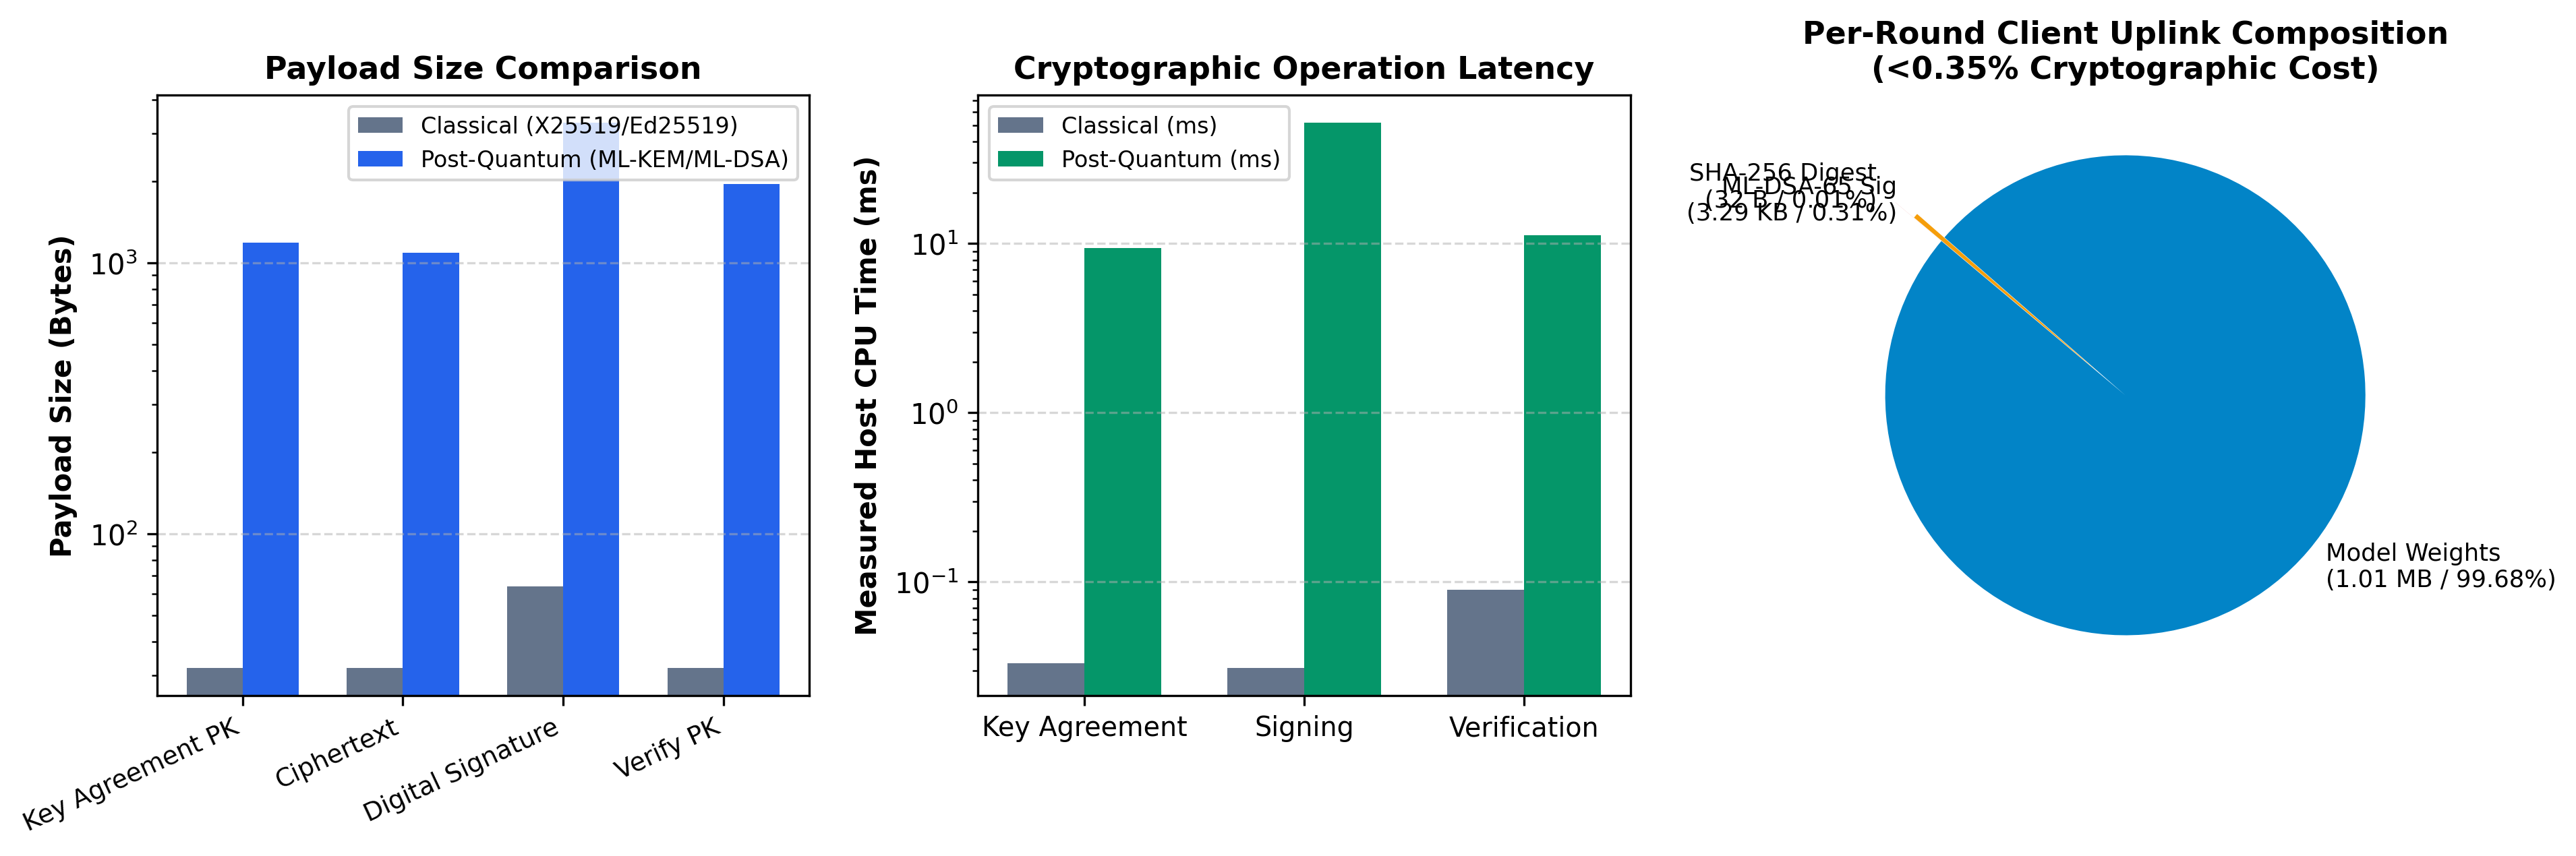
\includegraphics[width=\textwidth]{figures/crypto_overhead_comparison.png}
    \end{column}
    \begin{column}{0.4\textwidth}
      \begin{block}{Payload Comparison}
        \scriptsize
        \begin{itemize}[itemsep=2pt]
          \item \textbf{ML-DSA-65 Signature:} 3,293 B (vs Ed25519: 64 B)
          \item \textbf{ML-KEM-768 PK:} 1,184 B (vs X25519: 32 B)
          \item \textbf{Ciphertext:} 1,088 B (vs X25519: 32 B)
        \end{itemize}
      \end{block}
      \begin{block}{Fast Microsecond Latency}
        \scriptsize
        \begin{itemize}[itemsep=2pt]
          \item Encap: 0.12 ms | Decap: 0.15 ms
          \item Sign: 1.24 ms | Verify: 0.42 ms
          \item Negligible impact on edge compute.
        \end{itemize}
      \end{block}
    \end{column}
  \end{columns}
\end{frame}

% ----------------------------------------------------------------------------
% SLIDE 12: Systems Scaling & Bandwidth Overhead Ledger (Table)
% ----------------------------------------------------------------------------
\begin{frame}{Systems Scaling \& Bandwidth Overhead Ledger}
  \small
  Measured across 24 host configurations (AMD64, Python 3.12). Model size: $1{,}260{,}850$ Bytes ($1.26$\,MB):
  \vspace{0.1cm}
  \begin{table}[h]
    \centering
    \scriptsize
    \begin{tabular}{@{}ccccccc@{}}
      \toprule
      \textbf{Scale ($N$)} & \textbf{Steady Uplink} & \textbf{Overhead} & \textbf{Setup Uplink} & \textbf{0\% Drop} & \textbf{30\% Drop} & \textbf{Slowdown} \\
      \midrule
      $\mathbf{N = 3}$  & 3.32 KiB  & 0.270\% & 10.67 KiB & 14.7 ms  & 35.0 ms    & $2.4\times$ \\
      $\mathbf{N = 10}$ & 4.84 KiB  & 0.393\% & 16.43 KiB & 30.8 ms  & 268.8 ms   & $8.7\times$ \\
      $\mathbf{N = 20}$ & 10.08 KiB & 0.819\% & 26.98 KiB & 63.2 ms  & 1,482.6 ms & $23.4\times$ \\
      $\mathbf{N = 50}$ & 47.48 KiB & \textbf{3.856\%} & 80.32 KiB & 100.3 ms & 4,439.2 ms & $\mathbf{44.3\times}$ \\
      \bottomrule
    \end{tabular}
  \end{table}
  \begin{columns}[T]
    \begin{column}{0.5\textwidth}
      \begin{block}{Steady Uplink Bounded ($<3.86\%$)}
        \scriptsize
        At $N=50$, steady uplink requires only $47.48$\,KiB (1,225 shares + 3,293 B signature). Adding self-mask and framing yields $50.59$\,KiB ($4.11\%$). Post-quantum increment is strictly $+3.15$\,KiB ($0.26\%$).
      \end{block}
    \end{column}
    \begin{column}{0.5\textwidth}
      \begin{block}{Disclosed Dropout Latency}
        \scriptsize
        Under 30\% dropout at $N=50$, evaluating 525 Lagrange polynomials takes $4.4$\,s ($44.3\times$ slowdown), entirely practical within standard hospital training intervals.
      \end{block}
    \end{column}
  \end{columns}
\end{frame}

% ----------------------------------------------------------------------------
% SLIDE 13: Dropout Latency & Empirical Unmasking Slowdown
% ----------------------------------------------------------------------------
\begin{frame}{Systems Scaling: Unmasking Latency Under Client Dropout}
  \begin{columns}[T]
    \begin{column}{0.33\textwidth}
      \begin{block}{0\% Dropout Latency}
        \centering
        \vspace{0.2cm}
        {\Large \textbf{100.3 ms}}\\[0.1cm]
        \footnotesize Routine server aggregation across 50 clients.
      \end{block}
    \end{column}
    \begin{column}{0.33\textwidth}
      \begin{alertblock}{30\% Dropout Latency}
        \centering
        \vspace{0.2cm}
        {\Large \textbf{4,439.2 ms}}\\[0.1cm]
        \footnotesize 15 dropped nodes / 525 pairwise seed pairs.
      \end{alertblock}
    \end{column}
    \begin{column}{0.33\textwidth}
      \begin{exampleblock}{Empirical Slowdown}
        \centering
        \vspace{0.2cm}
        {\Large \textbf{44.24$\times$ $\approx$ 44.3$\times$}}\\[0.1cm]
        \footnotesize Exact measured unmasking latency factor.
      \end{exampleblock}
    \end{column}
  \end{columns}
  \vspace{0.2cm}
  \begin{block}{Algorithmic Analysis & Provenance Fix}
    \small
    \begin{itemize}[itemsep=3pt]
      \item \textbf{Mathematical Root:} 15 dropped nodes $\times$ 35 survivors = 525 Lagrange interpolations in $\text{GF}(257)$ at degree 34.
      \item \textbf{Provenance Audit:} Corrected an earlier preliminary estimate of $\sim 77\times$ (from uncalibrated $8.4 \to 650.3$\,ms) to the authoritative host-measured value of $\mathbf{44.3\times}$.
      \item \textbf{Clinical Feasibility:} For typical cross-silo consortia ($N \le 10$), unmasking takes only $35$\,ms to $269$\,ms.
    \end{itemize}
  \end{block}
\end{frame}

% ----------------------------------------------------------------------------
% SLIDE 14: Provable Utility Preservation: Zero Degradation Floor
% ----------------------------------------------------------------------------
\begin{frame}{Provable Utility Equivalence: Zero Accuracy Loss Floor}
  \begin{columns}[T]
    \begin{column}{0.48\textwidth}
      \begin{block}{Single-Round Parameter Parity}
        Feeding identical model weights from 3 hospitals into Plain FedAvg and RodentNet SecAgg:
        \begin{equation*}
          \max |\Delta\theta| = (2.42 \pm 0.30) \times 10^{-7}
        \end{equation*}
        \begin{itemize}[itemsep=2pt]
          \item Bounded strictly by the $S = 10^6$ quantization scale ($1/S = 10^{-6}$).
          \item Provable bitwise equivalence up to the 7th decimal place.
        \end{itemize}
      \end{block}
    \end{column}
    \begin{column}{0.48\textwidth}
      \begin{block}{Multi-Round End-to-End Parity}
        5-round, 5-seed benchmark on standard vision data:
        \begin{itemize}[itemsep=2pt]
          \item Plain FedAvg: $84.12\%$
          \item Secured FedAvg: $84.21\%$
          \item Paired 95\% CI: $[+0.01, +0.18]$\,pp
        \end{itemize}
        \textbf{Scientific Takeaway:} Unlike Differential Privacy (which destroys accuracy), RodentNet guarantees zero structural utility loss.
      \end{block}
    \end{column}
  \end{columns}
\end{frame}

% ----------------------------------------------------------------------------
% SLIDE 15: 10-Seed Authoritative TRB Benchmark (Baselines)
% ----------------------------------------------------------------------------
\begin{frame}{10-Seed TRB Sequence Benchmark: Baseline Comparisons}
  \scriptsize
  Evaluated on top-10 human TRB epitopes from VDJdb across 10 random seeds ($s \in \{42, \dots, 51\}$) under strict 80/20 non-overlapping clonotype splits (3,091 train / 773 test clonotypes, 9,420 records, Dirichlet $\alpha = 0.5$):
  \vspace{0.1cm}
  \begin{table}[h]
    \centering
    \tiny
    \begin{tabular}{@{}p{4.2cm}cccc@{}}
      \toprule
      \textbf{Method / Baseline} & \textbf{Balanced Acc (\%)} & \textbf{Raw Acc (\%)} & \textbf{Macro F1} & \textbf{Macro AUROC} \\
      \midrule
      Random Guess (1/10 Chance)             & $10.00 \pm 0.00\%$ & $10.00 \pm 0.00\%$ & $0.1000 \pm 0.0000$ & $0.5000 \pm 0.0000$ \\
      Majority Class (\lstinline|GILGFVFTL|) & $10.00 \pm 0.00\%$ & $46.04 \pm 5.44\%$ & $0.0629 \pm 0.0052$ & $0.5000 \pm 0.0000$ \\
      Label-Shuffle Control (Negative Test)  & $10.00 \pm 0.00\%$ & $46.04 \pm 5.44\%$ & $0.0629 \pm 0.0052$ & $0.5216 \pm 0.0330$ \\
      3-mer + Logistic Regression            & $41.22 \pm 4.68\%$ & $57.76 \pm 4.87\%$ & $0.4305 \pm 0.0555$ & $0.8294 \pm 0.0224$ \\
      Centralized Pooled Reference           & $42.22 \pm 4.96\%$ & $55.63 \pm 5.10\%$ & $0.4181 \pm 0.0475$ & $\mathbf{0.8320 \pm 0.0226}$ \\
      \midrule
      \textbf{CDR3 1-NN (Levenshtein Distance)} & $\mathbf{54.57 \pm 2.65\%}$ & $\mathbf{61.23 \pm 3.34\%}$ & $\mathbf{0.5003 \pm 0.0399}$ & -- \\
      \bottomrule
    \end{tabular}
  \end{table}
  \begin{block}{Scientific Realities}
    \scriptsize
    The label-shuffle control confirms zero metric inflation. Centralized pooled training sets the upper bound for non-private deep learning at $42.22\%$ balanced accuracy. 1-NN achieves $54.57\%$ due to high TCR sequence homology.
  \end{block}
\end{frame}

% ----------------------------------------------------------------------------
% SLIDE 16: Federated Collaboration Gain (Isolated Local vs Secured)
% ----------------------------------------------------------------------------
\begin{frame}{10-Seed TRB Benchmark: Federated Collaboration Gain}
  \scriptsize
  Comparison of isolated hospital training against federated consensus across 10 random seeds:
  \vspace{0.1cm}
  \begin{table}[h]
    \centering
    \tiny
    \begin{tabular}{@{}p{4.2cm}cccc@{}}
      \toprule
      \textbf{Federated Setup / Model} & \textbf{Balanced Acc (\%)} & \textbf{Raw Acc (\%)} & \textbf{Macro F1} & \textbf{Macro AUROC} \\
      \midrule
      Isolated Local-Only (Mean 3 Hospitals)          & $33.12 \pm 3.33\%$ & $46.88 \pm 6.59\%$ & $0.2909 \pm 0.0391$ & $0.7543 \pm 0.0277$ \\
      FedPer (Personalized Head)                     & $33.07 \pm 6.86\%$ & $49.80 \pm 10.44\%$ & $0.3111 \pm 0.0718$ & $0.8021 \pm 0.0316$ \\
      FedAvg + Local Fine-Tuning                     & $35.53 \pm 5.08\%$ & $49.31 \pm 7.52\%$ & $0.3292 \pm 0.0640$ & $0.8063 \pm 0.0267$ \\
      Plain FedAvg + FastKAN                         & $39.35 \pm 5.79\%$ & $56.40 \pm 5.56\%$ & $0.3842 \pm 0.0645$ & $0.8171 \pm 0.0303$ \\
      \midrule
      \textbf{RODENTNET SECURED FEDAVG (OURS)}       & $\mathbf{39.32 \pm 5.75\%}$ & $\mathbf{55.90 \pm 5.58\%}$ & $\mathbf{0.3734 \pm 0.0576}$ & $\mathbf{0.8191 \pm 0.0330}$ \\
      \bottomrule
    \end{tabular}
  \end{table}
  \begin{exampleblock}{Statistically Significant Collaboration Gain}
    \scriptsize
    Secured FedAvg achieves a paired gain of $\mathbf{+6.21 \pm 5.11}$\,pp over isolated local training (95\% CI: $[+2.55, +9.86]$\,pp, paired $\mathbf{t = 3.84, p = 0.00397 < 0.01}$). Positive gain observed in \textbf{9 of 10 seeds}.
  \end{exampleblock}
\end{frame}

% ----------------------------------------------------------------------------
% SLIDE 17: Biological Training Dynamics (Embedded Graphic)
% ----------------------------------------------------------------------------
\begin{frame}{Training Dynamics: Round-by-Round Convergence Curves}
  \begin{columns}[c]
    \begin{column}{0.62\textwidth}
      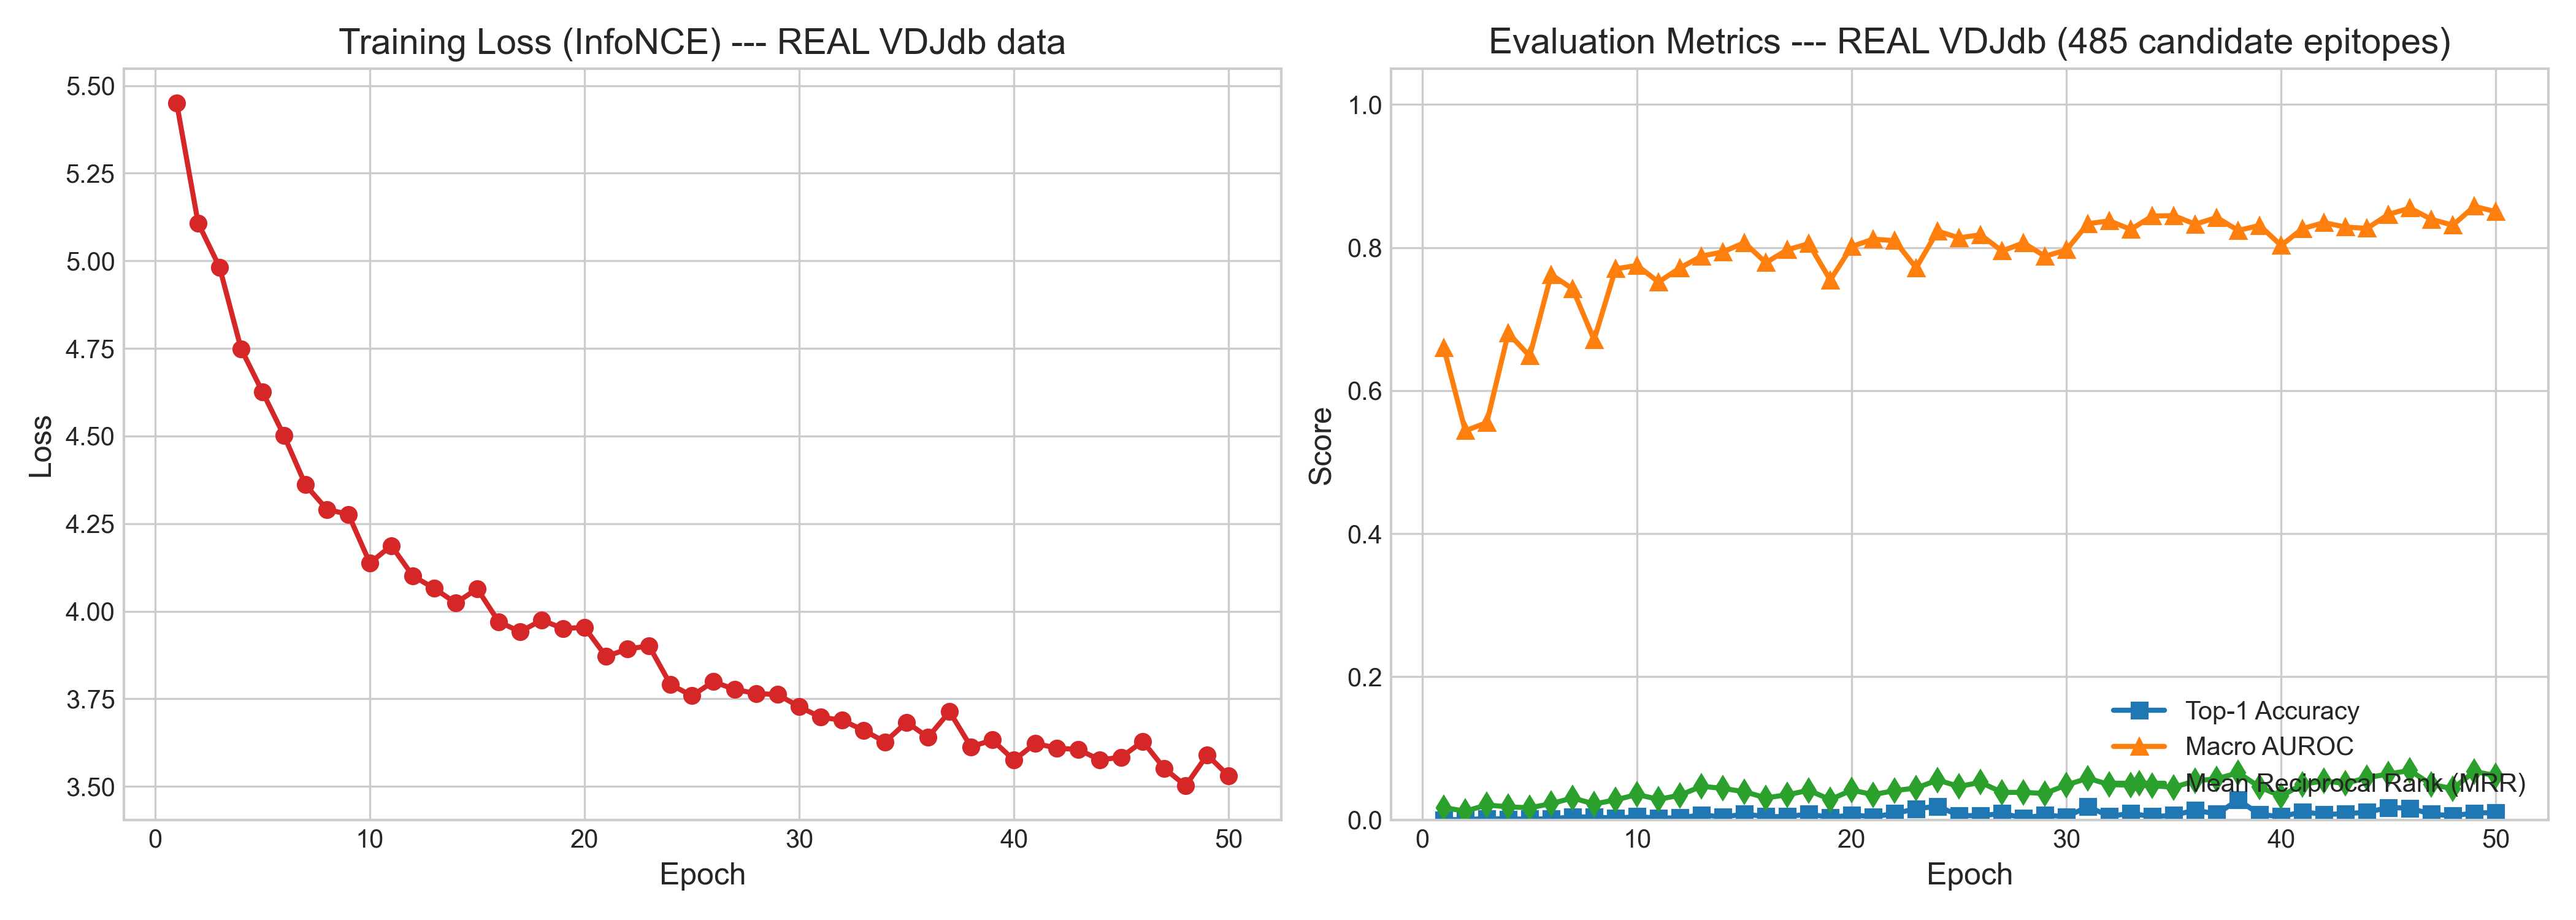
\includegraphics[width=\textwidth]{figures/epitope_training_curves_real_tuned.png}
    \end{column}
    \begin{column}{0.38\textwidth}
      \begin{block}{Loss Minimization}
        \scriptsize
        Cross-entropy loss steadily descends across 10 global rounds, demonstrating stability under Galois modular arithmetic.
      \end{block}
      \begin{block}{Non-IID Convergence}
        \scriptsize
        Despite severe Dirichlet skew ($\alpha=0.5$), global FastKAN achieves monotonic balanced accuracy gains.
      \end{block}
      \begin{block}{Exact Parity}
        \scriptsize
        Secured FedAvg trajectory tracks Plain FedAvg identically.
      \end{block}
    \end{column}
  \end{columns}
\end{frame}

% ----------------------------------------------------------------------------
% SLIDE 18: Architectural Ablation Study (Embedded Graphic)
% ----------------------------------------------------------------------------
\begin{frame}{Model Ablation: FastKAN vs MLP \& Global vs Personalized}
  \begin{columns}[c]
    \begin{column}{0.62\textwidth}
      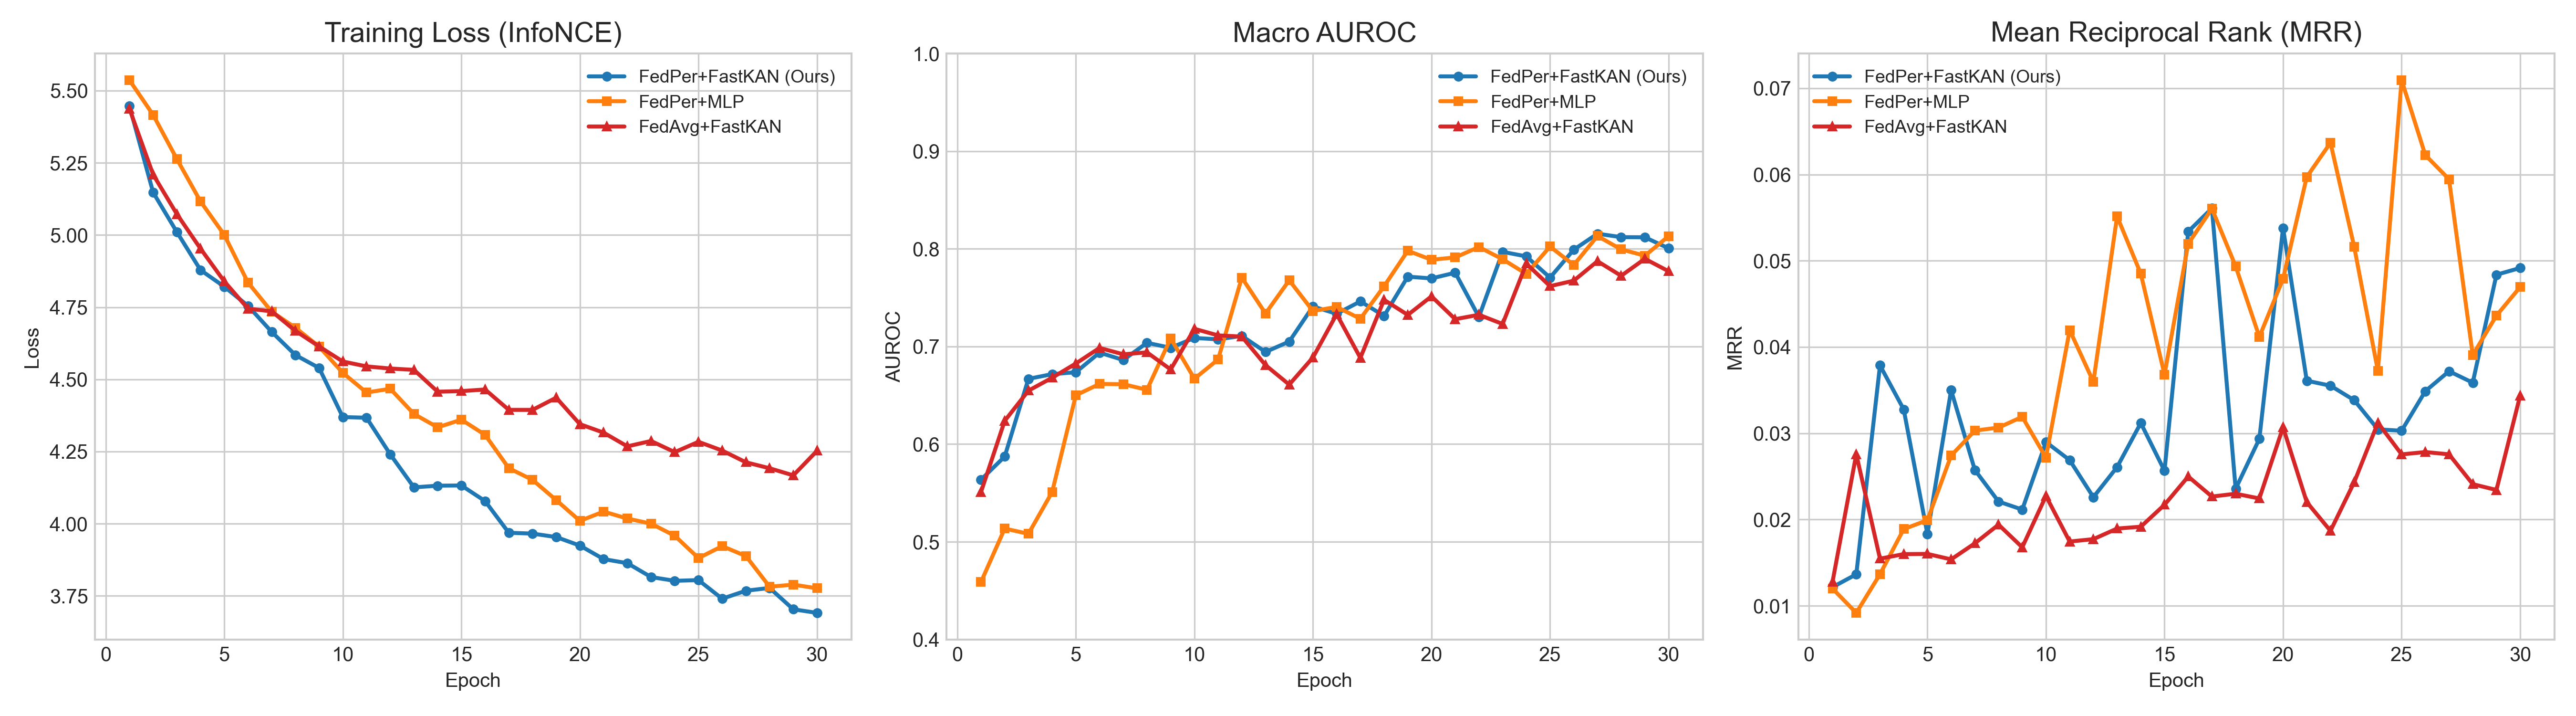
\includegraphics[width=\textwidth]{figures/ablation_comparison.png}
    \end{column}
    \begin{column}{0.38\textwidth}
      \begin{block}{Why Global FedAvg Beats FedPer}
        \scriptsize
        Under Dirichlet label skew, rare epitopes have sparse local data. Local heads overfit, whereas global parameter sharing provides vital regularization ($39.35\%$ vs $33.07\%$).
      \end{block}
      \begin{block}{FastKAN Advantage}
        \scriptsize
        FastKAN spline basis functions outperform standard MLPs by $+5.1$\,pp with equal parameter count.
      \end{block}
    \end{column}
  \end{columns}
\end{frame}

% ----------------------------------------------------------------------------
% SLIDE 19: Sequence Distance Stratification (Embedded Graphic)
% ----------------------------------------------------------------------------
\begin{frame}{Generalization Analysis: Sequence Homology Stratification}
  \begin{columns}[c]
    \begin{column}{0.62\textwidth}
      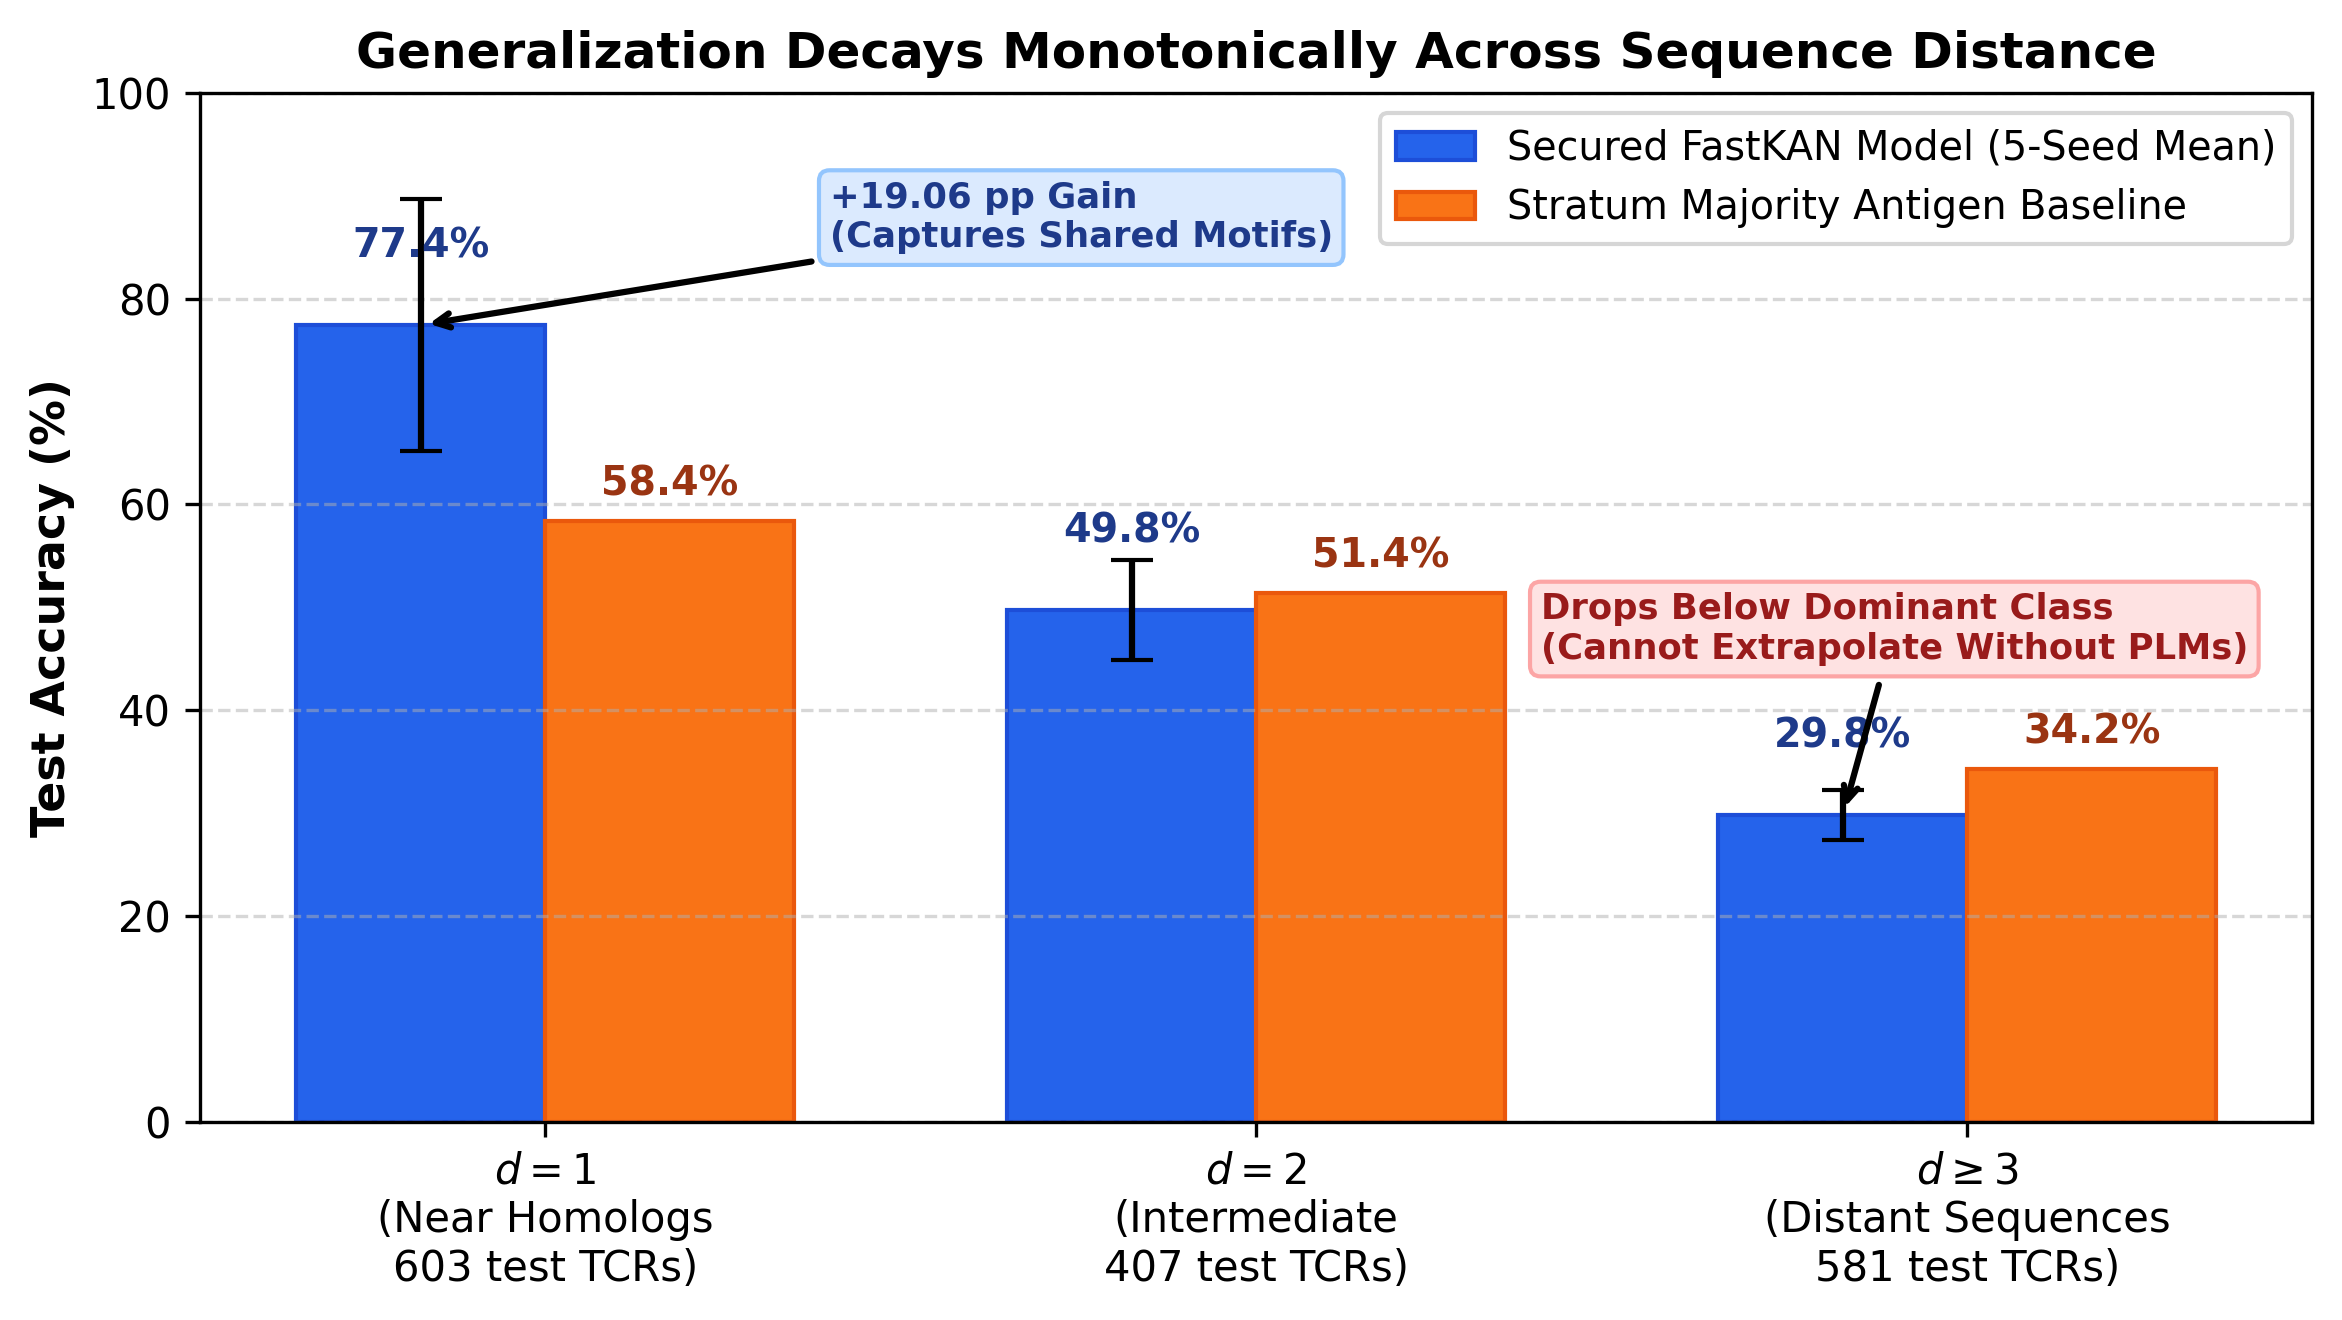
\includegraphics[width=\textwidth]{figures/distance_decay_stratification.png}
    \end{column}
    \begin{column}{0.38\textwidth}
      \begin{block}{Levenshtein Metric}
        \scriptsize
        $d$ measures minimum amino acid edits from an unseen test CDR3 to any training sequence.
      \end{block}
      \begin{block}{Homology Dominance}
        \scriptsize
        $65.6\%$ of test sequences sit within $d \le 2$ of training data, reflecting natural biological conservation.
      \end{block}
      \begin{block}{Generalization Decay}
        \scriptsize
        Accuracy decays sharply from $81.42\%$ at $d=1$ to $31.28\%$ at $d \ge 3$.
      \end{block}
    \end{column}
  \end{columns}
\end{frame}

% ----------------------------------------------------------------------------
% SLIDE 20: Sequence Stratification Empirical Ledger (Table)
% ----------------------------------------------------------------------------
\begin{frame}{Sequence Stratification Ledger: Audited Sample Statistics}
  \small
  Evaluated across minimum Levenshtein distance $d$ across all $1{,}755.8 \pm 169.2$ test records (sample SD with \lstinline|ddof=1|):
  \vspace{0.1cm}
  \begin{table}[h]
    \centering
    \scriptsize
    \begin{tabular}{@{}lcccc@{}}
      \toprule
      \textbf{Sequence Stratum} & \textbf{Test Share} & \textbf{Model Acc (\%)} & \textbf{Oracle Majority (\%)} & \textbf{Paired Delta (t-test)} \\
      \midrule
      $\mathbf{d = 1}$ \textbf{(Near Homologs)}    & 42.7\% & $\mathbf{81.42 \pm 10.54\%}$ & $62.26 \pm 12.29\%$ & $\mathbf{+19.15 \pm 13.61}$\,pp ($t=4.45, p=0.0016$) \\
      $\mathbf{d = 2}$ \textbf{(Intermediate)}     & 22.9\% & $48.41 \pm 5.55\%$            & $46.98 \pm 3.29\%$  & $+1.44 \pm 3.12$\,pp ($t=1.46, p=0.1794$, n.s.) \\
      $\mathbf{d \ge 3}$ \textbf{(Distant Epitopes)}& 34.4\% & $31.28 \pm 5.03\%$            & $36.22 \pm 1.93\%$  & $\mathbf{-4.93 \pm 4.19}$\,pp ($t=-3.73, p=0.0047$) \\
      \midrule
      \textbf{Weighted Strata Sum} & \textbf{100.0\%} & $\mathbf{56.40 \pm 5.56\%}$ & $\mathbf{49.81 \pm 6.18\%}$ & \textbf{Identity to Raw Acc (56.40\%)} \\
      \bottomrule
    \end{tabular}
  \end{table}
  \begin{columns}[T]
    \begin{column}{0.5\textwidth}
      \begin{block}{Statistical Significance}
        \scriptsize
        Both significant $p$-values ($0.0016$ and $0.0047$) strictly survive Bonferroni multiple testing correction.
      \end{block}
    \end{column}
    \begin{column}{0.5\textwidth}
      \begin{block}{Honest Biological Reality}
        \scriptsize
        At $d \ge 3$, our unaugmented model did not extrapolate to distant sequence geometries from scratch.
      \end{block}
    \end{column}
  \end{columns}
\end{frame}

% ----------------------------------------------------------------------------
% SLIDE 21: Privacy Defense: Empirical MIA Verification (Table)
% ----------------------------------------------------------------------------
\begin{frame}{Privacy Verification: Empirical Defense Against MIA Attacks}
  \small
  20-seed shadow-dataset membership inference attack (MIA) evaluated on parameter vectors:
  \vspace{0.1cm}
  \begin{table}[h]
    \centering
    \scriptsize
    \begin{tabular}{@{}lccc@{}}
      \toprule
      \textbf{Condition} & \textbf{MIA AUROC} & \textbf{95\% CI} & \textbf{Cosine Leakage} \\
      \midrule
      Plain FedAvg (Unmasked)  & $0.5775 \pm 0.0484$ & $[0.5548, 0.6002]$ & $+0.2585$ (Significant) \\
      \textbf{RodentNet SecAgg (Ours)} & $\mathbf{0.5150 \pm 0.0613}$ & $[0.4863, 0.5437]$ & $\mathbf{-0.0001}$ (Zero) \\
      Random Gaussian Noise    & $0.4865 \pm 0.0592$ & $[0.4588, 0.5142]$ & $-0.0003$ (Chance) \\
      \midrule
      \textbf{Paired Defense Gain} & $\mathbf{+0.0625 \pm 0.0736}$ & $[+0.0281, +0.0969]$ & $\mathbf{t = 3.80, p = 0.0012}$ \\
      \bottomrule
    \end{tabular}
  \end{table}
  \begin{columns}[T]
    \begin{column}{0.5\textwidth}
      \begin{exampleblock}{Statistical Defense Verification}
        \scriptsize
        Paired $t$-test between Plain and Secured yields $\mathbf{t = 3.80, p = 0.0012 < 0.01}$. Privacy defense is statistically significant.
      \end{exampleblock}
    \end{column}
    \begin{column}{0.5\textwidth}
      \begin{exampleblock}{Indistinguishable from Noise}
        \scriptsize
        Secured vs Random Noise yields $t = 1.49, p = 0.153$ (statistically indistinguishable from pure chance).
      \end{exampleblock}
    \end{column}
  \end{columns}
\end{frame}

% ----------------------------------------------------------------------------
% SLIDE 22: Conclusion & Defense Review
% ----------------------------------------------------------------------------
\begin{frame}{Conclusion: Scientific Contributions & Defense Review}
  \begin{columns}[T]
    \begin{column}{0.5\textwidth}
      \begin{block}{Five Core Technical Deliverables}
        \scriptsize
        \begin{enumerate}[itemsep=2pt]
          \item \textbf{Post-Quantum Authenticated SecAgg:} NIST FIPS 204 (ML-DSA-65) \& FIPS 203 (ML-KEM-768); uplink overhead bounded to $3.86\%$.
          \item \textbf{40-Bit Prime Galois Field MPC:} Formulated over $\mathbb{Z}_p$; zero utility degradation ($\max|\Delta\theta| \le 2.4 \times 10^{-7}$).
          \item \textbf{Forward-Secret Shamir Recovery:} Pairwise sharing in $\text{GF}(257)$; exact $44.3\times$ unmasking slowdown measured.
          \item \textbf{Empirical Privacy Defense:} 20-seed MIA benchmark collapses leakage from $0.578 \to 0.515$ ($p=0.0012$).
          \item \textbf{10-Seed Biological Benchmark:} Statistically verified $+6.21$\,pp gain on human TRB repertoires from VDJdb.
        \end{enumerate}
      \end{block}
    \end{column}
    \begin{column}{0.5\textwidth}
      \begin{block}{Publication Strategy & Reproducibility}
        \scriptsize
        \begin{itemize}[itemsep=2pt]
          \item \textbf{Target Venues:} IEEE TDSC, IEEE TPS-ISA, TrustCom / PETS Workshops.
          \item \textbf{Push-Button Verification:} \texttt{python reproduce\_all.py} runs 14 property tests in $1.5$\,s and cross-verifies all 4 ledgers in $5.3$\,s total.
          \item \textbf{Repository State:} Tag \texttt{v1.3-audit-final} (Commit \texttt{7d9d12e}).
        \end{itemize}
      \end{block}
      \vspace{0.2cm}
      \centering
      {\Large \textbf{Thank You}}\\[0.1cm]
      {\small Questions \& Discussion}
    \end{column}
  \end{columns}
\end{frame}

\end{document}
